\subsubsection{Mechanism for pushing button}
\paragraph{Plan of creating module:}	
	
	\begin{enumerate}
		\item Creating 3D model in Creo parametric.
		\item Calculaition distances and angels.
		\item  Programming and debugging the mechanism
	\end{enumerate}
	The module represents the servo, which turns the beam. The beam can push right and left button. Also the module includes Hi-Technic colour sensor, which can detect the colour of the button.	
  \begin{figure}[H]
		\begin{minipage}[h]{\linewidth}
			\center{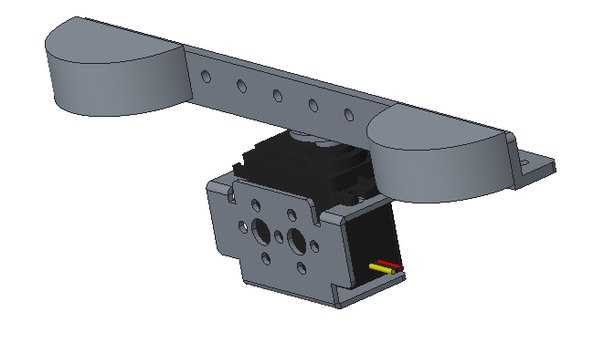
\includegraphics[scale=0.5]{3Engineering/6Specifications_for_modules/button/images/01}}
			\caption{Creo model}
		\end{minipage}
	\end{figure}
  \begin{figure}[H]
		\begin{minipage}[h]{\linewidth}
			\center{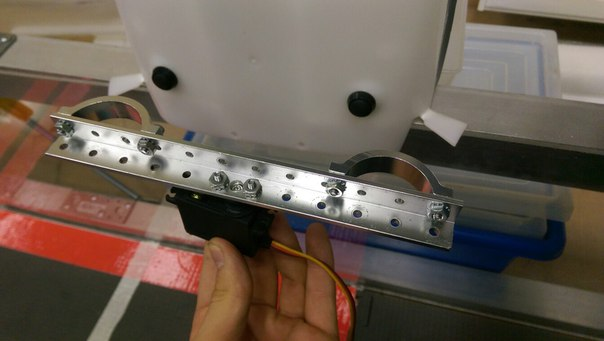
\includegraphics[scale=0.5]{3Engineering/6Specifications_for_modules/button/images/02}}
			\caption{Real model}
		\end{minipage}
	\end{figure}
	
	\paragraph{Algorithm}
	
	\begin{enumerate}	
		\item At first, the robot stops near the button. Then the sensor detects the colour of right button. If the colour is similar to our colour of alliance then the servo turns and the beam pushes the right button. In other case, servo turns in another direction and pushes the left button.  
	\end{enumerate}
	
	\paragraph{Programming}
 
	 To detect the colour of the button we use the algorithm of colour focus. Every colour has 3 parameters: red, green and blue. These three parameters can be represented as the basis of a 3-axis coordinate system. We need two vectors шт this coordinate system: one from calibration procedure and one measured during the game. Than we calculate the angle between them. If the angle value is below special limit, we can conclude that the measured colour is similar to calibrated one.
	 \begin{figure}[H]
	 	\begin{minipage}[h]{\linewidth}
	 		\center{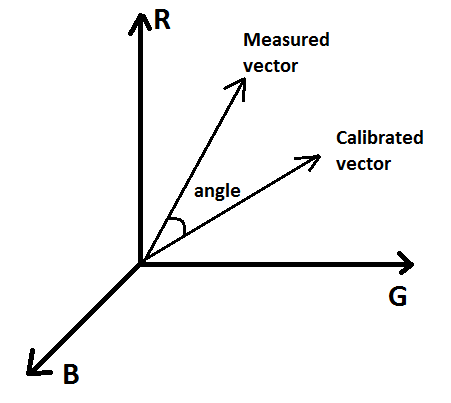
\includegraphics[scale=0.7]{3Engineering/6Specifications_for_modules/button/images/04}}
	 		\caption{Colour focus}
	 	\end{minipage}
	\end{figure}

	\fillpage
